\section{Strategie di distribuzione}
In questa sezione vengono esposte le scelte progettuali di distribuzione.\\
\subsection{Due possibili strategie di distribuzione}
\label{scelted}
Nella simulazione del traffico di una città ciò che ragionevolmente potrebbe trarre vantaggi dalla distribuzione sta nella segmentazione della dimensione della città, al fine di poter distribuire su più nodi parti di una stessa città che si vuole simulare. Seguendo questo approccio quindi la città risulterebbe suddivisa in quartieri e ogni quartiere rappresenterebbe quindi parte dell'intera mappa della città, suddividendo cosi su più nodi il luogo della realizzazione dello spostamento delle entità. \\
Un'altra possibile strategia potrebbe essere quella di conservare in un unico luogo la mappa e quindi centralizzando su un nodo lo stato di avanzamento del sistema. Questa strategia non gode tuttavia della proprietà della scalabilità della mappa; cioè come si comporterebbe il sistema nel caso cambiasse la configurazione della mappa della città da simulare se la città fosse di dimensioni notevoli? D'altro canto questa strategia semplificherebbe di molto la gestione dell'orologio virtuale per l'avanzamento delle entità del tipo veicolo, bici o pedone dato che tutto secondo la strategia in questione diviene centralizzato; seguendo questa strategia la distribuzione potrebbe ricadere non più sulla mappa ma sulle entità da spostare; tuttavia il nodo che conserva l'intera mappa diverrebbe un collo di bottiglia per gli aggiornamenti di stato delle entità. \\
\subsection{Strategia di distribuzione scelta}
La strategia scelta è stata la prima esposta in \ref{scelted} dato che sfrutta bene il concetto della distribuzione permettendo così la gestione dei calcoli per l'avanzamento delle entità e delle richieste su più nodi.

\subsection{Definizione dei ruoli delle entità del sistema}
Le entità esposte in \ref{firstmappa} meritano un ruolo in funzione della strategia di distribuzione scelta. Fondamentalmente le entità in un sistema concorrente e distribuito vengono distinte in attive e reattive. \\
Ponendo il ruolo di entità attiva sulle entità del tipo veicolo, bici o pedoni si presenterebbe un problema relativo allo spostamento delle entità nel caso queste debbano muoversi tra un quartiere e l'altro; ovvero, dato che le entità attive richiedono un processo, questo significa che nel momento in cui un'entità debba essere spostata tra due quartieri si avrebbe un processo inutile instanziato in un quartiere e occorrerebbe instanziare un processo nel quartiere di destinazione della entità; questo potrebbe essere un problema dato che vengono instanziati dinamicamente dei processi e quindi si potrebbero ottenere errori a run-time nel caso in cui il nodo non riesca ad instanziare il nuovo processo; l'alternativa potrebbe essere preallocare un certo numero di thread per ospitare le entità che richiedono di essere spostate nel quartiere interessato; a questo punto però occorrerebbe porre una limitazione sul numero di entità che un certo quartiere potrebbe ospitare; questo risulerebbe quindi poco scalabile e scomodo da gestire dato che si potrebbe avere un'entità in attesa di essere spostata su un quartiere affinchè questo liberi un thread dal proprio thread-pool di risorse preallocate. \\
Il ruolo di entità attiva dovrebbe ricadere quindi sulle entità di tipo strada o incrocio. Dato che la mappa presenta, una volta configurata e istanziata, una configurazione stabile si avrà che il sistema non instanzierà dinamicamente dei processi; inoltre ogni partizione per soddisfare le richieste di altre partizioni se dotata di un thread-pool risolve anche il problema dell'allocazione di thread per richieste remote da soddisfare.\\
Seguendo questa strategia il sistema diviene scalabile sia in termini di distribuzione che di concorrenza.

\subsection{Componenti oggetto della distribuzione}\label{subsec:distribuzione}
\begin{figure}[H] % Example image
\center{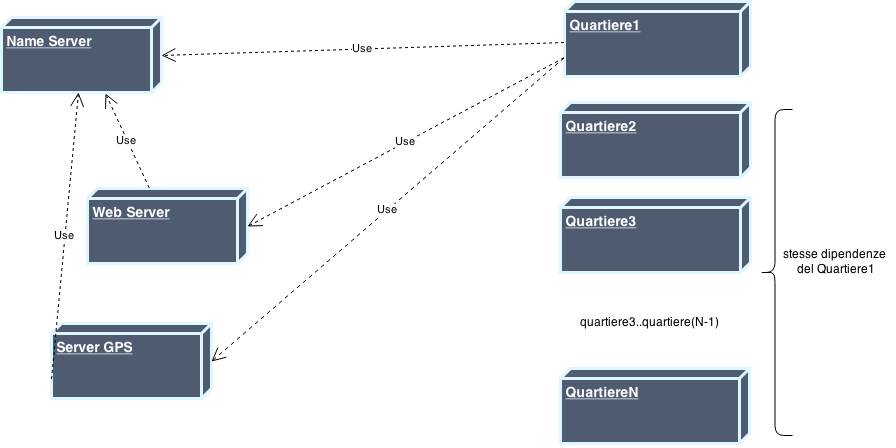
\includegraphics[width=1.0\linewidth]{DiagrammaComponenti}}
\caption{Diagramma componenti.}
\label{fig:Diagramma componenti}
\end{figure}
In questa sezione vengono descritte le componenti del sistema:
\begin{itemize}
\item un quartiere è una componente che deve essere istanziata per ogni frammento della mappa previsto dalla configurazione; se un quartiere presenta una configurazione valida, esso può entrare a far parte del sistema in qualunque momento (entro il limite previsto del numero massimo di quartieri instanziabili). Un quartiere è responsabile dello spostamento delle entità che sono in transito in una qualunque delle strade o incroci che appartegono al quartiere stesso. Le entità reattive quali i veicoli, le bici e i pedoni vengono instanziate in uno specifico quartiere e le informazioni relative allo stato del percorso di queste entità saranno sempre reperibili dal quartiere al quale l'entità è stata instanziata, al fine di evitare che nel momento in cui un'entità debba essere spostata da un quartiere all'altro, non occorra riportare tutto lo stato del percorso al quartiere interessato.\\
Dato che una volta configurato il sistema le entità reattive non cambiano in numero e contenuto informativo, conviene riportare per ogni quartiere una cache delle entità di ogni altro quartiere al fine di evitare un numero eccessivo di richieste a quartieri remoti responsabili dell'istanziazione delle entità interessate durante le fase di avanzamento delle entità;
\item il server GPS è una componente passiva che si occupa del calcolo del percorso per conto di una entità. Questa componente dispone della conoscenza della mappa di ogni quartiere correttamente istanziato. Il server GPS effettua un'aggiornamento della mappa in relazione alle nuove richieste di istanziazione di nuovi quartieri. Il calcolo del percorso avviene eseguendo l'algoritmo di Dijkstra dei cammini minimi. Se una certa entità deve muoversi verso una certa destinazione non ancora raggiungibile, a causa del fatto che il quartiere interessato non è stato ancora istanziato occorrerà ritardare lo spostamento dell'entità. Il server per una stessa entità potrebbe calcolare percorsi minimi diversi per 2 richieste diverse nel caso in cui nel frattempo è stato istanziato un nuovo quartiere che presenta un percorso più breve per raggiungere la destinazione;
\item il web server è quella componente responsabile della creazione della view e del rendering dello stato di avanzamento delle entità del sistema;
\item il name server si occupa invece di servire alle altre partizioni richieste di accesso e riferimento a risorse che risiedono su una partizione remota.
\end{itemize}